% ---------------------------------------------------------------------------
%  Academic poster: A1 portrait, three columns
%  Built with the tcolorbox poster library (bundled), no extra poster class.
%  Each \posterbox is one panel; move panels with column= / span= / below= / between=.
%  Text is TeX Gyre Heros (bundled), so any size scales cleanly; plots use pgfplots.
%  The study and its numbers are fictional examples.
% ---------------------------------------------------------------------------
\documentclass{article}

\usepackage[a1paper,portrait,margin=2.2cm]{geometry}
\usepackage{lmodern} % scalable maths at poster sizes; load before fontspec
\usepackage{fontspec}
\setmainfont{texgyreheros}[
  Extension=.otf, UprightFont=*-regular, ItalicFont=*-italic,
  BoldFont=*-bold, BoldItalicFont=*-bolditalic]
\usepackage{amsmath}
\usepackage{graphicx}
\usepackage{booktabs}
\usepackage{enumitem}
\usepackage{pgfplots}
\pgfplotsset{compat=1.18}
\usepackage[most]{tcolorbox}
\tcbuselibrary{poster}

% A dark neutral for structure, one green accent
\definecolor{ink}{HTML}{1F3A33}
\definecolor{accent}{HTML}{2F7D63}
\definecolor{mist}{HTML}{75837E}
\definecolor{paper}{HTML}{F4F7F5}

\pagestyle{empty}
\setlist{nosep, leftmargin=1.1em, itemsep=.35em, label={\color{accent}\rule[.25ex]{.45em}{.45em}}}
\pgfplotsset{every axis/.append style={
  axis lines=left, axis line style={mist, line width=1.5pt}, tick style={mist, line width=1.5pt},
  tick label style={font=\fontsize{24}{28}\selectfont, /pgf/number format/assume math mode=true},
  scale only axis, label style={font=\fontsize{26}{30}\selectfont},
  legend style={draw=none, fill=none, font=\fontsize{24}{28}\selectfont}}}

\begin{document}
\fontsize{32}{44}\selectfont
\color{ink}\raggedright

\begin{tcbposter}[
  coverage = {spread, colback=white},
  poster = {columns=3, rows=12, spacing=1.4cm},
  boxes = {enhanced, sharp corners, boxrule=0pt, colback=white, colframe=white,
           coltitle=accent, colbacktitle=white,
           fonttitle=\bfseries\fontsize{40}{48}\selectfont\raggedright,
           before upper=\raggedright,
           left=0pt, right=0pt, top=8pt, bottom=12pt, toptitle=14pt, bottomtitle=10pt,
           borderline north={2pt}{0pt}{ink}},
]

% ---------------------------------------------------------------- title
\posterbox[blankest, valign=center]{name=title, column=1, span=3, below=top}{%
  {\fontsize{30}{36}\selectfont\bfseries\color{accent}RESEARCH POSTER\par}
  \vspace{.4em}
  {\bfseries\fontsize{104}{116}\selectfont The Quiet Page\par}
  \vspace{.15em}
  {\fontsize{50}{60}\selectfont Line length, leading, and the speed of reading on screens\par}
  \vspace{.8em}
  {\fontsize{34}{42}\selectfont Mira Okafor\textsuperscript{1}\quad Tomás Ilves\textsuperscript{2}\quad Hana Sato\textsuperscript{1}\par}
  {\fontsize{28}{36}\selectfont\color{mist}\textsuperscript{1}Reading Lab, Northfield University\qquad
    \textsuperscript{2}Institute for Visual Communication\qquad mira.okafor@northfield.edu\par}
}

% ---------------------------------------------------------------- takeaway (bottom band)
\posterbox[blankest, interior engine=path, colback=paper, interior style={fill=paper},
  left=1.2cm, right=1.2cm, top=.9cm, bottom=.9cm]{name=takeaway, column=1, span=3, above=bottom}{%
  {\fontsize{30}{36}\selectfont\bfseries\color{accent}TAKEAWAY\par}\vspace{.3em}
  {\fontsize{46}{58}\selectfont Cap the measure at about \textbf{66 characters}. Add leading only when a
    long line cannot be avoided: it helps long lines, never short ones.\par}
}

% ---------------------------------------------------------------- column 1
\posterbox[adjusted title=Why it matters]{name=why, column=1, below=title}{
  Most advice on line length was formed on paper, a century ago. Today the same text is read on
  phones, laptops and wide monitors, and the reader can resize the window at will.
  \par\vspace{.6em}
  We ask a simple question: \emph{does the old rule still hold on screens?}
}

\posterbox[adjusted title=What we did]{name=method, column=1, below=why}{
  \begin{itemize}
    \item 312 adults, 24 short essays each
    \item 6 line lengths, 35--115 characters
    \item 4 line spacings, 1.0--1.6
    \item Speed on first read, then four comprehension questions
  \end{itemize}
  \vspace{.6em}
  A mixed model with random intercepts for reader and essay:
  \begin{align*}
    \log \mathrm{wpm} &= \beta_0 + f(L) + \beta_s S \\
                       &\quad + \beta_{Ls} L S + u_i + v_e .
  \end{align*}
}

\posterbox[adjusted title=References]{name=refs, column=1, above=takeaway}{
  {\fontsize{24}{32}\selectfont\color{mist}
  [1] R.\,Bringhurst. \emph{The Elements of Typographic Style}. 2004.\par
  [2] M.\,A.\,Tinker, D.\,G.\,Paterson. Length of line. \emph{J. Appl. Psych.}, 1929.\par
  [3] M.\,C.\,Dyson. Text layout and reading from screen. \emph{BIT}, 2004.\par}
}

\posterbox[adjusted title=At a glance]{name=glance, column=1, between=method and refs}{
  \vfill
  {\fontsize{60}{68}\selectfont\bfseries\color{accent}312\par}
  {\color{mist}readers, 7\,488 essays read\par}
  \vfill
  {\fontsize{60}{68}\selectfont\bfseries\color{accent}+20\%\par}
  {\color{mist}speed at 66 vs.\ 105 characters\par}
  \vfill
}

% ---------------------------------------------------------------- columns 2--3
\posterbox[adjusted title=Speed peaks near 66 characters per line]{name=result, column=2, span=2, below=title}{
  \begin{center}
  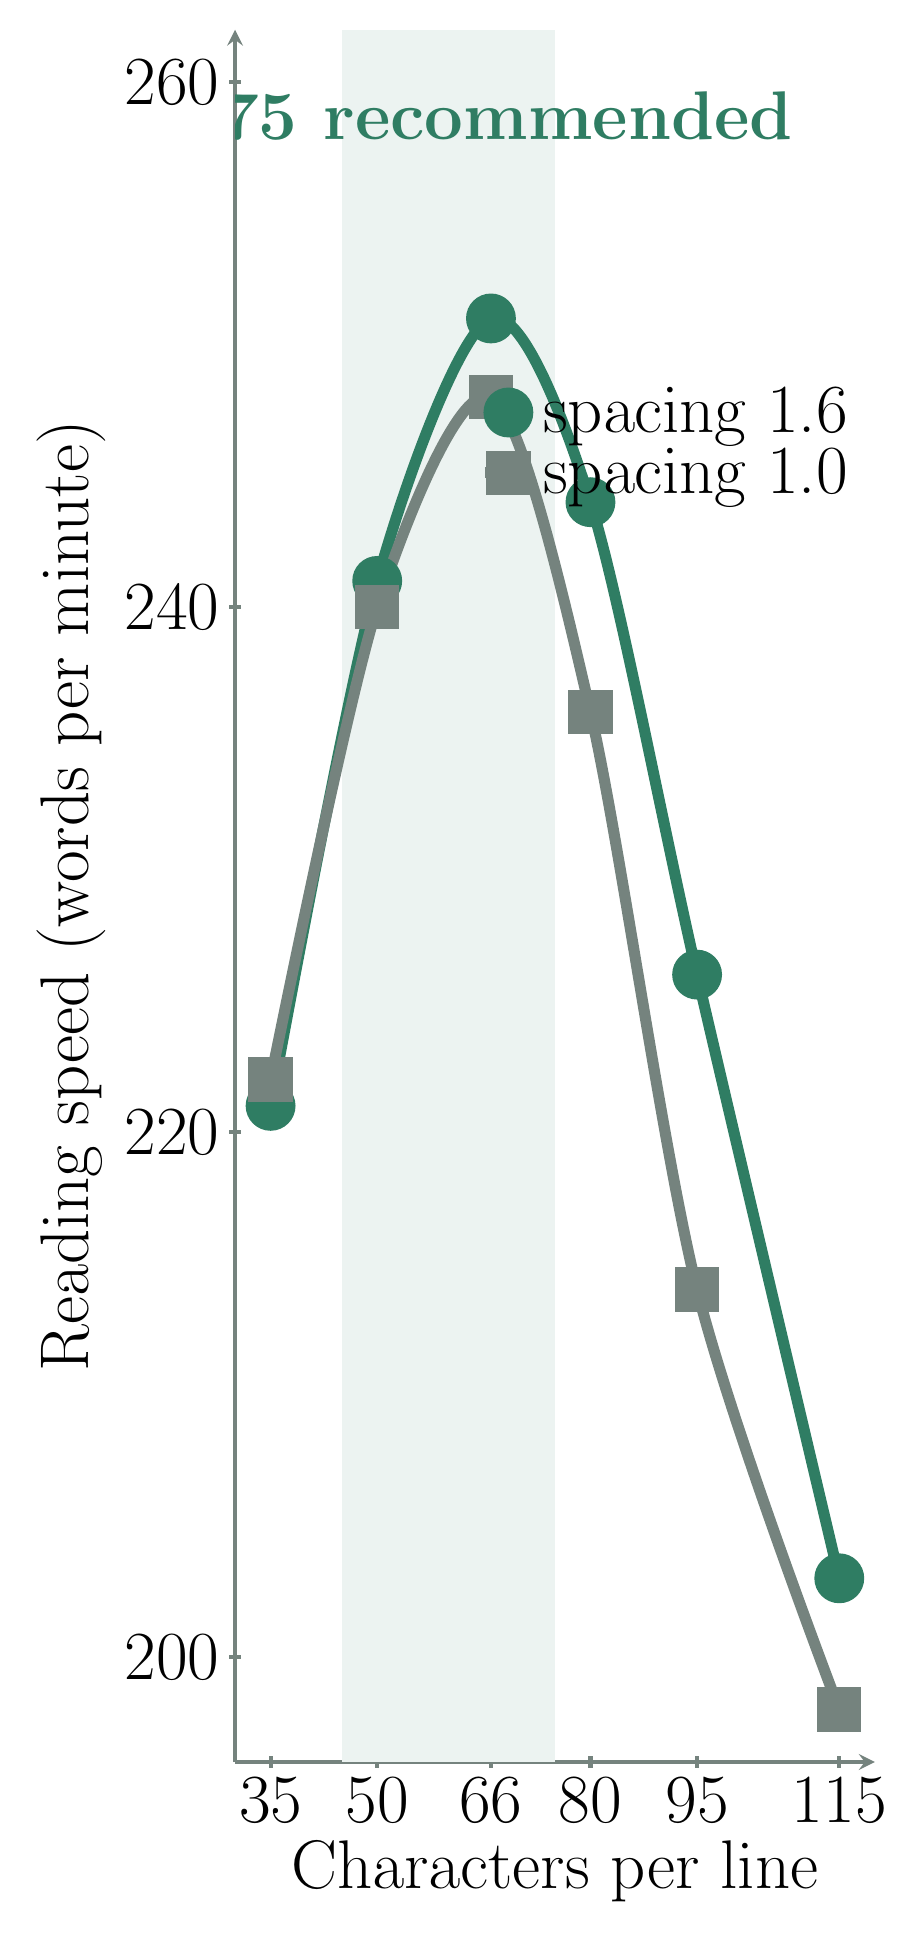
\begin{tikzpicture}
    \begin{axis}[
      width=\linewidth-4cm, height=22cm,
      xlabel={Characters per line}, ylabel={Reading speed (words per minute)},
      xmin=30, xmax=120, ymin=196, ymax=262, ytick={200,220,240,260},
      xtick={35,50,66,80,95,115},
      legend style={at={(0.98,0.80)}, anchor=north east},
      every axis plot/.append style={line width=4pt, smooth},
    ]
      \fill[accent!9] (axis cs:45,196) rectangle (axis cs:75,262);
      \node[font=\fontsize{24}{28}\selectfont\bfseries, text=accent, anchor=north] at (axis cs:60,260) {45--75 recommended};
      \addplot[accent, mark=*, mark size=7pt] coordinates
        {(35,221) (50,241) (66,251) (80,244) (95,226) (115,203)};
      \addlegendentry{spacing 1.6}
      \addplot[mist, mark=square*, mark size=6pt] coordinates
        {(35,222) (50,240) (66,248) (80,236) (95,214) (115,198)};
      \addlegendentry{spacing 1.0}
    \end{axis}
  \end{tikzpicture}
  \end{center}
}

\posterbox[adjusted title=Understanding stays flat]{name=compr, column=2, between=result and takeaway}{
  Readers did not understand less on long lines; they worked harder to understand the same.
  \par\vspace{.8em}
  \begin{center}
  \renewcommand{\arraystretch}{1.3}
  \begin{tabular}{@{}l r r@{}}
    \toprule
    Line length & Speed & Correct \\
    \midrule
    35  & 221 & 86\% \\
    66  & \textbf{\color{accent}250} & 87\% \\
    105 & 209 & 85\% \\
    \bottomrule
  \end{tabular}
  \end{center}
  \vfill
  {\bfseries Which page did readers prefer?\par}
  \vspace{.5em}
  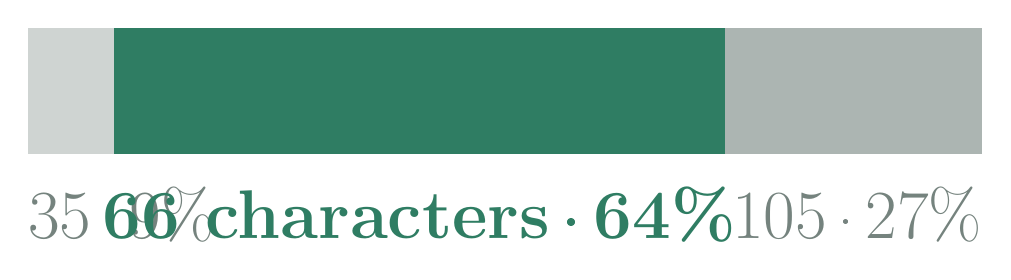
\begin{tikzpicture}[x=\linewidth/100]
    \fill[mist!35] (0,0) rectangle (9,1.6);
    \fill[accent] (9,0) rectangle (73,1.6);
    \fill[mist!60] (73,0) rectangle (100,1.6);
    \node[anchor=north west, inner xsep=0pt, font=\fontsize{24}{28}\selectfont, text=mist] at (0,-.3) {35\,·\,9\%};
    \node[anchor=north, font=\fontsize{24}{28}\selectfont\bfseries, text=accent] at (41,-.3) {66 characters\,·\,64\%};
    \node[anchor=north east, inner xsep=0pt, font=\fontsize{24}{28}\selectfont, text=mist] at (100,-.3) {105\,·\,27\%};
  \end{tikzpicture}
  \vfill
}

\posterbox[adjusted title=Leading helps long lines only]{name=leading, column=3, between=result and takeaway}{
  \begin{center}
  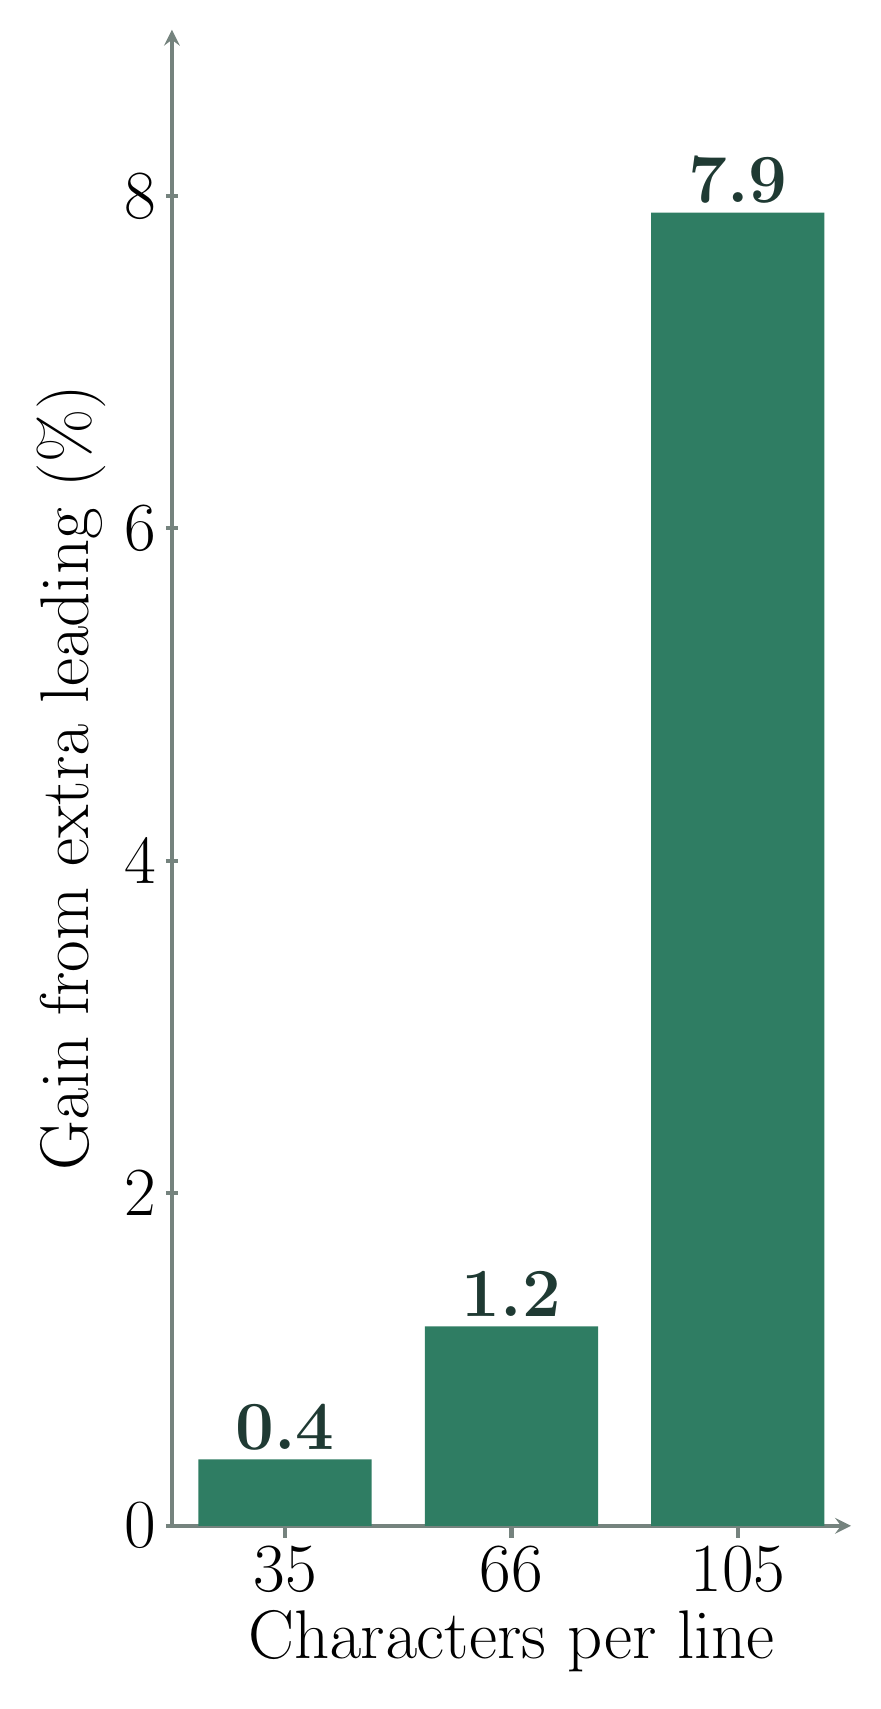
\begin{tikzpicture}
    \begin{axis}[
      width=\linewidth-3.5cm, height=19cm, ybar, bar width=2.2cm,
      symbolic x coords={35,66,105}, xtick=data,
      xlabel={Characters per line}, ylabel={Gain from extra leading (\%)},
      ymin=0, ymax=9, ytick={0,2,4,6,8},
      nodes near coords, nodes near coords style={font=\fontsize{24}{28}\selectfont\bfseries, text=ink, /pgf/number format/assume math mode=true},
      enlarge x limits=.25,
    ]
      \addplot[fill=accent, draw=none] coordinates {(35,0.4) (66,1.2) (105,7.9)};
    \end{axis}
  \end{tikzpicture}
  \end{center}
}

\end{tcbposter}
\end{document}
